\RequirePackage{fix-cm}
%
\RequirePackage{amsmath}



%\documentclass{svjour3}                     % onecolumn (standard format)
%\documentclass[smallcondensed]{svjour3}     % onecolumn (ditto)
%\documentclass[smallextended]{svjour3}       % onecolumn (second format)
% \documentclass[twocolumn]{svjour3}          % twocolumn
%\documentclass[letterpaper, 12pt, twocolumn]{article}
\documentclass{article}
\usepackage[cm]{fullpage}
%\usepackage[margin=1in]{geometry}
\usepackage{amssymb}
\usepackage{graphicx}
\usepackage[utf8]{inputenc}
\usepackage{indentfirst}
%\usepackage{physics}
\newcommand{\me}{\mathrm{e}}
\usepackage{amsmath}

%\usepackage[monochrome]{color}

%\usepackage[round]{natbib}
%\usepackage{apacite}
\usepackage{url}


\PassOptionsToPackage{monochrome}{xcolor}

% For the flow charts
\usepackage{tikz}
\usetikzlibrary{
	external,
}
\tikzexternalize

\usetikzlibrary{shapes.geometric, arrows, calc, positioning}
\tikzstyle{startstop} = [rectangle, thick, rounded corners=2.5mm, minimum width=2cm, minimum height=5mm,text centered, draw=black]
\tikzstyle{io} = [trapezium, thick, trapezium left angle=70, trapezium right angle=110, text width=3.75cm, minimum height=0.5cm, text centered, draw=black]
\tikzstyle{process} = [rectangle, thick, minimum width=2.5cm, text width=4cm, minimum height=0.5cm, text centered, draw=black]
\tikzstyle{block} = [rectangle, thick, minimum width=0.5cm, minimum height=1cm, text centered, draw=black]
\tikzstyle{support} = [coordinate, join=by fuzzy]
\tikzstyle{decision} = [diamond, thick, minimum width=3cm, minimum height=1cm, text centered, draw=black]
\tikzstyle{dottedbox} = [rectangle, dotted, thick, minimum width=2.5cm, text width=2.8cm, minimum height=0.5cm, text centered, draw=black]
\tikzstyle{arrow} = [thick,->,>=stealth]
\tikzstyle{dottedarrow} = [thick, dotted,->,>=stealth]





\usepackage{pgfplots}
\usepgfplotslibrary{patchplots}
\pgfplotsset{compat=newest, samples=015} %Set this value to 65 for the final version
%\usepgfplotslibrary{dateplot} 


%\providecommand{\keywords}[1]{\textbf{\textit{Index terms---}} #1}

%\journalname{Journal of Science Education and Technology}

\begin{document}


\title{Algorithm to generate multi-factorial experiments to teach experimental design%\thanks{Grants or other notes
%about the article that should go on the front page should be
%placed here. General acknowledgments should be placed at the end of the article.}
}
%\subtitle{Do you have a subtitle?\\ If so, write it here}
%\titlerunning{Short form of title}        % if too long for running head
\author{A.C.~Delgado-Chavez  \and
        N.~Balagurusamy \and
        R.~Narayanasamy \and
        S.~K.~Gadi
}

\begin{figure}
	\centering
	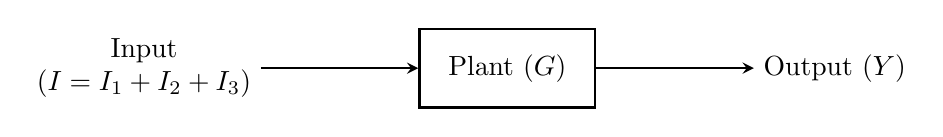
\begin{tikzpicture}[node distance = 10mm, auto]
		\node (Input) [align=center] {Input\\($I=I_1+I_2+I_3$)};
		\node (Plant) [block, text width = 2cm, right = 2cm of Input] {Plant ($G$)};
		\node (Output) [right = of Plant, right = 2cm] {Output ($Y$)};
		\draw [arrow] (Input) -- (Plant);
		\draw [arrow] (Plant) -- (Output);
	\end{tikzpicture}
	\caption{Open loop system}
	\label{Fig:OpenLoop}
\end{figure}

\pagebreak
\begin{figure}
	\centering
	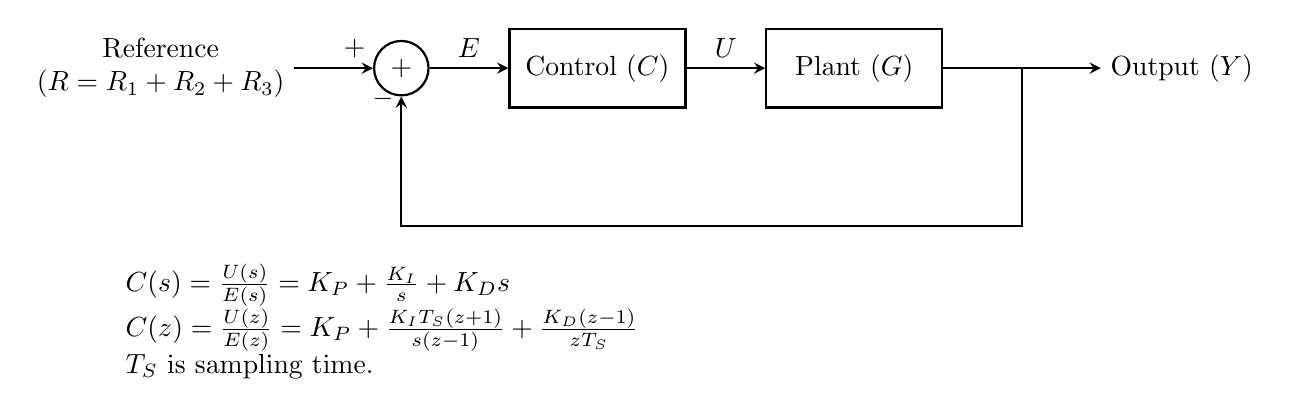
\begin{tikzpicture}[node distance = 10mm, auto]
	\node (Reference) [align=center] {Reference\\($R=R_1+R_2+R_3$)};
	\node (SummingPoint) [draw,circle, thick, right = of Reference]  {+};
	\node (Control) [block, text width = 2cm, right = of SummingPoint] {Control ($C$)};
	\node (Plant) [block, text width = 2cm, right = of Control] {Plant ($G$)};
	\node (PlantRight) [support, right = of Plant, right = 1cm] {};
	\node (Output) [right = of Plant, right = 2cm] {Output ($Y$)};
	\draw [arrow] (Reference) -- node[anchor=south west]{+}(SummingPoint);
	\draw [arrow] (SummingPoint) -- node[anchor=south]{$E$}(Control);
	\draw [arrow] (Control) -- node[anchor=south]{$U$}(Plant);
	\draw [arrow] (Plant) -- (Output);
	\draw [arrow] (PlantRight) -- +(0, -2) -| (SummingPoint) node[below = 2mm, anchor=north east]{\bf\textendash};
	\node (Equation000) [text width = 7cm, below = 2cm of SummingPoint, align = left] {
		$C(s) = \frac{U(s)}{E(s)} = K_P + \frac{K_I}{s} + K_Ds$\\
		$C(z) = \frac{U(z)}{E(z)} = K_P + \frac{K_IT_S(z+1)}{s(z-1)} + \frac{K_D(z-1)}{zT_S}$\\
		$T_S$ is sampling time.
	};
	\end{tikzpicture}
	\caption{Closed loop system with a PID Controller}
	\label{Fig:PID}
\end{figure}

\pagebreak
\begin{figure}
	\centering
	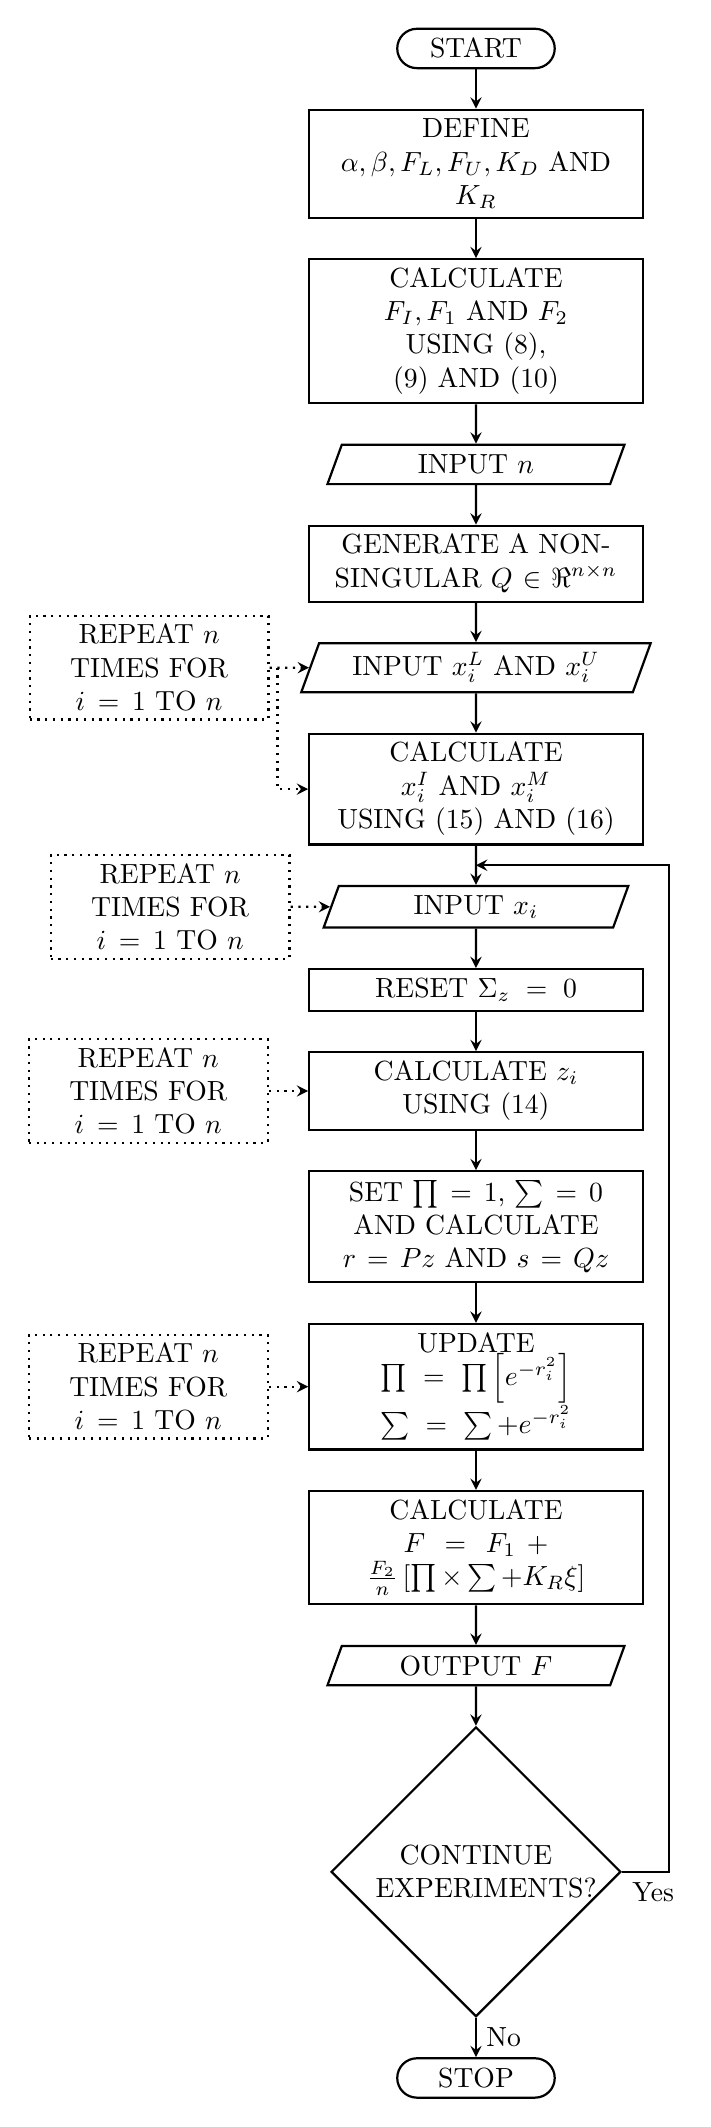
\begin{tikzpicture}[node distance = 5mm, auto]
		\node (Start) [startstop] {START};
		\node (Define) [process, below = of Start] {DEFINE $\alpha, \beta, F_L, F_U, K_D$~AND $K_R$};
		\node (Calculate01) [process, below =of Define] {CALCULATE\\$F_I, F_1$ AND $F_2$\\USING (8), (9) AND (10)};
		\node (Input01) [io, below = of Calculate01, text width=3cm] {INPUT $n$};
		\node (Calculate01a) [process, below = of Input01] {GENERATE A NONSINGULAR $Q\in \Re^{n\times n}$};
		\node (Input02) [io, below = of Calculate01a] {INPUT $x_i^L$~AND~$x_i^U$};
		\node (Calculate02) [process, below = of Input02] {CALCULATE\\$x_i^I$ AND $x_i^M$\\USING (15) AND (16)};
		\node (Input03) [io, below = of Calculate02, text width=3.25cm] {INPUT $x_i$};
		\node (Calculate03) [process, below = of Input03] {RESET $\Sigma_z=0$};
		\node (Calculate04) [process, below = of Calculate03] {CALCULATE $z_i$\\ USING (14)};
		\node (Calculate05) [process, below = of Calculate04] {SET $\prod=1$, $\sum = 0$ \\AND CALCULATE \\ $r=Pz$ AND $s=Qz$};
		\node (Calculate06) [process, below = of Calculate05] {UPDATE\\ $\prod = \prod \left[e^{-r_i^2}\right]$\\$\sum=\sum + e^{-r_i^2}$};
		\node (Calculate07) [process, below = of Calculate06] {CALCULATE \\ $F=F_1+\frac{F_2}{n}\left[\prod \times \sum + K_R\xi\right]$};
		\node (Output03) [io, below = of Calculate07, text width=3cm] {OUTPUT $F$};
		\node (Decision01) [decision, below = of Output03, text width=2.55cm] {CONTINUE\\EXPERIMENTS?};
		\node (Stop) [startstop, below = of Decision01] {STOP};

		\node (ForBox01) [dottedbox, left = of Input02, left = 5mm] {REPEAT $n$ TIMES FOR $i=1$ TO $n$};
		%\node (ForBox02) [dottedbox, left of=Calculate02, left = 2.25cm] {REPEAT $n$ TIMES FOR $i=1$ TO $n$};
		\node (ForBox03) [dottedbox, left = of Input03, left = 5mm] {REPEAT $n$ TIMES FOR $i=1$ TO $n$};
		\node (ForBox04) [dottedbox, left = of Calculate04, left = 5mm] {REPEAT $n$ TIMES FOR $i=1$ TO $n$};
		\node (ForBox05) [dottedbox, left = of Calculate06, left = 5mm] {REPEAT $n$ TIMES FOR $i=1$ TO $n$};

 		%\node (stop) [startstop, below of=calculate1, below = 0mm] {STOP};
		\draw [arrow] (Start) -- (Define);
		\draw [arrow] (Define) -- (Calculate01);
		\draw [arrow] (Calculate01) -- (Input01);
		\draw [arrow] (Input01) -- (Calculate01a);
		\draw [arrow] (Calculate01a) -- (Input02);
		\draw [arrow] (Input02) -- (Calculate02);
		\draw [arrow] (Calculate02) -- (Input03);
		\draw [arrow] (Input03) -- (Calculate03);
		\draw [arrow] (Calculate03) -- (Calculate04);
		\draw [arrow] (Calculate04) -- (Calculate05);
		\draw [arrow] (Calculate05) -- (Calculate06);
		\draw [arrow] (Calculate06) -- (Calculate07);
		\draw [arrow] (Calculate07) -- (Output03);
		\draw [arrow] (Output03) -- (Decision01);
		\draw [arrow] (Decision01) -- node[anchor=west]{No}(Stop);
		\draw [arrow] ($ (Decision01.east) $)node[anchor=north west]{Yes}  -- ++(0.6,0.00) |- ($ (Input03.north) + (0mm,2.5mm) $);

		\draw [dottedarrow] (ForBox01) -- (Input02);
		%\draw [dottedarrow] (ForBox02) -- (Calculate02);
		\draw [dottedarrow] ($(ForBox01.east) + (1mm,0mm)$) |- (Calculate02);
		\draw [dottedarrow] (ForBox03) -- (Input03);
		\draw [dottedarrow] (ForBox04) -- (Calculate04);
		\draw [dottedarrow] (ForBox05) -- (Calculate06);
	\end{tikzpicture}
	\caption{Flowchart of the proposed algorithm}
	\label{Fig:AlgorithmInFlowchart}
\end{figure}



%\bibliographystyle{apacite}%unsrtnat}
%\bibliographystyle{spbasic}      % basic style, author-year citations
%\bibliographystyle{spmpsci}      % mathematics and physical sciences
%\bibliographystyle{spphys}       % APS-like style for physics
%\bibliographystyle{ieeetr}
%\bibliography{refs}
\end{document}